\chapter{Present research}\label{present-research}

In this chapter we offer an overview of the recent research in the field of signed graphs. 

\section{Chromatic number}

Now we will explore some properties of the chromatic number of signed graphs as defined by Máčajová et. al. We briefly summarize the results, the proofs can be found in \cite{chromatic-number}.
If $(G, \Sigma)$ has a positive loop, a proper coloring is not possible. So for the rest of this section we assume
only graphs without positive loops. It is also good to keep in mind that the color $0$ behaves differently from the other colors, because $0 = -0$. 
(For example if there is a negative loop at a vertex $v$, then $\phi (v) \neq 0$.)
First, let's compare the chromatic number of a signed graph to the chromatic number of its underlying graph.

\begin{theorem}[Máčajová et. al.]
    For every loopless signed graph $(G, \Sigma)$ we have

    $$\chi ((G, \Sigma)) \leq 2 \chi (G) - 1$$

    Furthermore, this boundary is sharp.
\end{theorem}

The idea for the first part is that each coloring of $G$ using colors in $\{0, 1, \dots, n-1\}$
is also a signed coloring of $(G, \Sigma)$ using colors from $\{0, \pm 1, \pm 2, \dots, \pm (n-1)\} = M_{2n-1}$.

A signed graph is antibalanced if the sign product on every even circuit is positive and on every odd circuit negative.
(Each such graph is equivalent to an all-negative signature). Based on \cref{vertex-set-partition}, we can partition the 
vertex set of an antibalanced signed graph into two sets such that each edge with one end in the first set and the other end in the second set is positive and edges inside the sets are negative.
An antibalanced signed graph has to be bipartite, so antibalanced signed graphs are a natural generalization of bipartite graphs.

\begin{proposition}[Máčajová et. al.]
    A signed graph is 2-colorable ($\chi ((G, \Sigma)) \leq 2$) if and only if it is antibalanced.
\end{proposition}

If the graph is antibalanced, we can switch some vertices to make it all-negative and color all vertices $1$.
If the graph is 2-colorable, we can partition the vertices into positive ($V_1$) and negative ($V_{-1}$).
The edges within the sets have to be negative and edges between the sets have to be positive, which fits the definition of an antibalanced graph.

\begin{proposition}[Máčajová et. al.]
    If $(G, \Sigma)$ is a signed complete graph on $n$ vertices, then $\chi ((G, \Sigma)) \leq n$. 
    Furthermore, $\chi ((G, \Sigma)) = n$ if and only if $(G, \Sigma)$ is balanced.
\end{proposition}

\cite{chromatic-number} proves the Brooks' theorem\cite{brooks} for signed graphs and concludes by proving the five color theorem for planar signed graphs.
Let's observe the maximmum degree $\Delta$ of signed graphs with regard to the chromatic number.
If we color the vertices greedily using any ordering of the vertices, for each vertex at most
$\Delta$ colors are taken by previous neighbors. Hence $\chi ((G, \Sigma)) \leq \Delta + 1$. 
The maximum chromatic number $\Delta + 1$ is reached in case of a balanced complete graph and
a balanced odd ciricuit, similar to the unsigned version. There is one more signed case, however: even unbalanced circuits.

\begin{theorem}[Máčajová et. al.]
    Let $(G, \Sigma)$ be a simple connected signed graph. If $(G, \Sigma)$ is not a balanced complete graph,
    a balanced odd circuit or an unbalanced even circuit, then $\chi ((G, \Sigma)) \leq \Delta (G)$.
\end{theorem}

($\Delta (G)$ is the maximum degree of $G$)

In this article Máčajová et. al. also conjectured that the 4-color-theorem is also true for signed graphs. However, this conjecture
was later disproved\cite{signed-4-color-conjecture}

\section{Nowhere-zero flows}

Nowhere-zero flows in signed graphs: A survey\cite{nowhere-zero-flows-survey} captures the recent knowledge about nowhere-zero flows and circuit covers in signed graphs.
There is a well-known duality between nowhere-zero flows and vertex coloring of unsigned planar graphs, which has been extended to signed graphs. 
They was originally introduced on signed graphs by Edmonds and Johnson\cite{edmonds-johnson} for expressing algorithms on matchings, but the first to systematically study this was Bouchet \cite{bouchet-flows}.
To understand
the problem of nowhere-zero flows on signed graphs, we first define \textit{signed circuits} (known to be the circuits of the associated signed graphic matroid). 
They are the equivalent of circuits on unsigned graphs for signed graphs. \cite{nowhere-zero-flows-survey} recognizes two types of signed circuits (\cref{fig:signed-circuits}):

\begin{itemize}
    \item balanced circuits
    \item barbells; the union of two unbalanced vertices connected by a (possibly trivial) path $P$ with endvertices $v_1 \in V(C_1)$ and $v_2 \in V(C_2)$ such that $C_1 - v_1$ is disjoint from $P \cup C_2$ and $C_2 - v_2$ is disjoint from $P \cup C_1$
\end{itemize}

We refer to the original, unsigned circuits as \textit{ordinary circuits}.

In order to assign signed edges an orientation, we perceive them as two half-edges. 
An \textit{orientation} of an edge $e$ consists of directions assigned to each half-edge of $e$ \cref{fig:edge-orientation}.
An edge is \textit{consistently oriented} if exactly one of the half-edges $h$, $h'$ making up $e$ points toward the corresponding endvertex.
If both of them point to their respective endvertex $e$ is \textit{extroverted} and if none of them does, $e$ is \textit{introverted}.
We say that an oriented edge is \textit{incoming} at a vertex $v$ if its half-edge incident with $v$ points towards $v$ and \textit{outgoing} at $v$ otherwise.

An \textit{orientation} (often referred to as \textit{bidirection}) of a signed graph $(G, \Sigma)$ is the assignment of orientation to each edge of $G$ in such a way that the positive edges
are exactly the consistently oriented ones. An oriented signed graph is also called an \textit{bidirected graph}.

\begin{figure}[ht]\label{fig:signed-circuits}
    \centering
    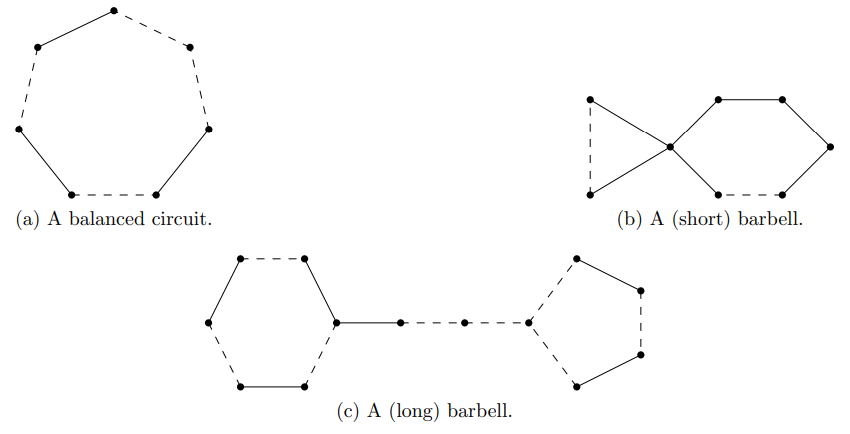
\includegraphics[scale=0.65]{images/signed-circuits.png}
    \caption{Signed circuits (dashed lines indicate negative edges)}
\end{figure}

\begin{figure}[ht]\label{fig:edge-orientation}
    \centering
    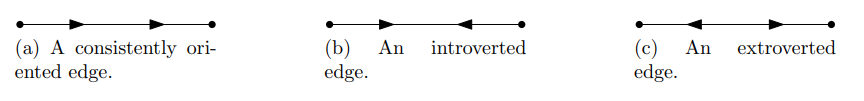
\includegraphics[scale=0.65]{images/oriented-edges.png}
    \caption{Edge orientation}
\end{figure}

\section{Nowhere-zero flows}

Let $\Gamma$ be an Abelian group. A $\Gamma$-flow in $(G, \Sigma)$ consists of an orientation of $(G, \Sigma)$ and 
a function $\phi : E(G) \rightarrow \Gamma$ such that the usual conservation law is satisfied: 
for each vertex $v$ the sum of $\phi (e)$ over the incoming edges $e$ equals the sum of $\phi (e)$ over the outgoing edges $e$\cite{nowhere-zero-flows-survey}.
A $\Gamma$-flow is \textit{nowhere-zero} if the value $0$ is never used for any edge.
A $\mathbb{Z}$-flow is said to be a $k$-flow ($k \geq 2$, $k$ is an integer) if for each edge $e$: $|\phi (e)| \leq k$.
If a signed graph $(G, \Sigma)$ admits a nowhere-zero $k$-flow, its \textit{flow-number} $\Phi (G, \Sigma)$ is defined as the smallest $k$ such that $(G, \Sigma)$ admits a nowhere-zero $k$-flow.
Otherwise $\Phi (G, \Sigma)$ is defined as $\infty$.

A signed graph is said to be \textit{flow-admissible} if it admits at least one nowhere-zero $\mathbb{Z}$-flow.

\begin{theorem}[Bouchet\cite{bouchet-flows}]
    A signed graph $(G, \Sigma)$ is flow-admissible if and only if each every edge of $(G, \Sigma)$ belongs to a signed circuit.
\end{theorem}

Nowhere-zero flows on signed graphs are a generalization of the same concept on unsigned graphs, 
because the definition of a flow on an all-positive signed graph corresponds to the definition of a flow on an unsigned graph.

Directly from the previous theorem follows 

\begin{corollary}\label{one-negative-edge-flow}
    A signed graph with one negative edge is not flow-admissible.
\end{corollary}

Tutte\cite{tutte-proof} proved that an unsigned graph $G$ admits a nowhere-zero $k$-flow if and only if it admits a nowhere-zero $\mathbb{Z}_k$ flow. 
However, this is not true for signed graphs in general. For example an unbalanced circuit admits a $\mathbb{Z}_2$-flow, but no integer flow.

Buchet stated the following conjecture, mirroring its importance with the similar Tutte's 5-flow conjecture.

\begin{conjecture}
    Every flow-admissible signed graph admits a nowhere-zero 6-flow.
\end{conjecture}

\begin{figure}[ht]\label{fig:no-5-flow}
    \centering
    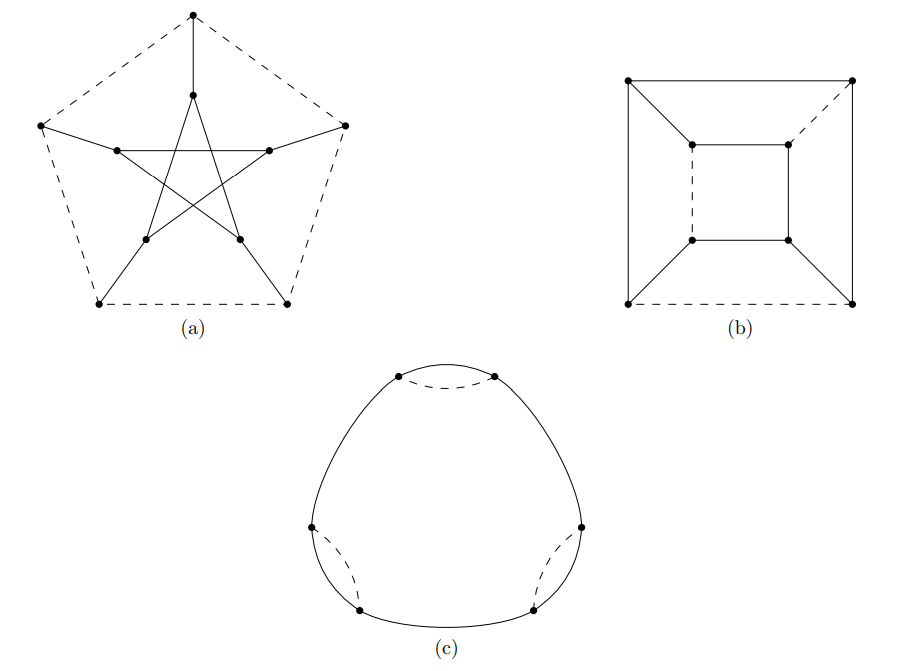
\includegraphics[scale=0.65]{images/petersen-no-5.png}
    \caption{Signed graphs with no nowhere-zero 5-flows}
\end{figure}

The value 6 would be best possible, since there exist graphs that admit no nowhere-zero 5-flows.
Bouchet originally also proved the theorem for value 216. This number was improved multiple times, 
the lowest value was proved by DeVos\cite{devos}.

\begin{theorem}[DeVos]
    Every flow-admissible signed graph admits a nowhere-zero 12-flow.
\end{theorem}

\section{Flows on signed cubic graphs}

In the field of signed regular graphs, most of the research is focused on signed cubic graphs and this will most likely be 
the focus of my thesis to some degree. Máčajová and Škoviera
characterized signed cubic graphs with flow number 3 or 4. In their Remarks on nowhere-zero flows in signed cubic graphs\cite{cubic-signed-graphs}
they investigate integer and group flows in signed graphs with the following results.

\begin{theorem}
    Let $(G, \Sigma)$ be a signed cubic graph. Then

    \begin{enumerate}
        \item [(i)] $(G, \Sigma)$ admits a nowhere-zero 3-flow if and only if it is antibalanced and has a perfect matching (or a 1-factor).
        \item [(ii)] $(G, \Sigma)$ admits a nowhere-zero $\mathbb{Z}_3$-flow if and only if it is antibalanced.
        \item [(iii)] $(G, \Sigma)$ admits a nowhere-zero $\mathbb{Z}_4$-flow if and only if it has an antibalanced 2-factor.
        \item [(iv)] $(G, \Sigma)$ admits a nowhere-zero $\mathbb{Z}_2 \times \mathbb{Z}_2$-flow if and only if $G$ is 3-edge-colourable. 
    \end{enumerate}
\end{theorem}

\section{Edge coloring on signed graphs}

Let $\Delta _G$ be the maximum degree among vertices of an ordinary graph $G$. According to Vizing's theorem, $G$ is $n$-edge-colorable, where $n$ is either $\Delta _G$
or $(\Delta _G + 1)$. In addition to defining edge coloring on signed graphs, Behr also proves the signed version of the Vizing's theorem.
Remember that edge coloring is an assignment of colors to edge-vertex incidences, not only edges. One of the consequences of this fact
is that signed Kempe chains (used to switch colors in the original Vizing's theorem) are not paths, but trails. The vertices in one chain may 
repeat with opposite colors. 

Behr shows that every signed edge coloring can be realised as a vertex coloring of a signed line graph.
Since unsigned edge coloring has this property, it is also desired in the signed version. 
A line graph of an ordinary graph has a vertex for each edge of the original graph and two vertices are connected if their corresponding edges were originally adjacent
In order to show this in signed graphs, we need to revisit bidirected graphs. Remember, that bidirected graphs are basically oriented signed graphs, the definition from the Flows section applies as well.
Positive edges are consistently oriented and negative edges are extroverted or introverted.
So every bidirected graph can be reverted back to an undirected signed graph based on the consistency of its edge orientations.

A proper coloring of a bidirected graph is an assignment of colors from $M_n$ to edges, \textit{not} edge-vertex incidences. 
There is no need to involve vertices, because the direction of half-edges for each vertex ensures vertex switching consistency, so only a single color is needed for each vertex.
Given an undirected signed graph and its edge coloring, this coloring uniquely determines edge colorings of each bidirected graph, that can be obtained by giving the original signed graph an orientation.
Consider the following coloring transformation. In the undirected graph, negative edges have the same color on both ends, let's say color $a$. So the color of the bidirected edge will be $a$ if it is extroverted and $-a$ if it is introverted.
Positive edges have opposite colors on their vertices. The bidirected edge will have the color "it points to", it will inherit the color from the vertex-edge incidence where the edge is incoming.
Now let's reorient an edge by inverting the orientation of both half-edges and the color. The bidirected coloring remains consistent with the orientation \textit{and} with the original undirected edge coloring.
So the bidirected coloring is determined uniquely by the original coloring and edge orientation and given two orientations $B$ and $B'$ with their respective colorings $\gamma _b$ and $\gamma _{B'}$ (originating from the same colored graph),
reorienting edges of $B$ to arrive at $B'$ also transforms $\gamma _B$ into $\gamma _{B'}$.

Consequently, the construction of a line graph through a bidirected graph does \textit{not} depend on the orientation. To create a signed line graph,
we pick any orientation $B$ of a signed graph $(G, \Sigma)$, then create a bidirected line graph. Each edge will become a vertex.
New vertices are connected if they previously shared a vertex and the orientation of these edges depends on the consistency of the corresponding half-edges in the previous graph.
If both edges were incoming or outgoing at their common vertex, the new edge between them will be negative, otherwise it will be positive. 
For the purposes of constructing a line graph we don't need to deduce the orientation of this line graph, as it will be discarded in the result anyway.

The vertex coloring of the line graph directly corresponds to the edge coloring of the bidirected graph, since the edges retain their color after becoming vertices.
So there is indeed a bijection between the edge coloring of a signed graph and the vertex coloring of its line graph.
